
La planificación temporal del Proyecto se basa en el tiempo que ha tomado realizar el Trabajo de Fin de Grado que envuelve este Proyecto, desde la toma de contacto con el director del Proyecto, hasta la finalización del mismo. La planificación se divide en varias etapas, pasando por el estudio de la situación actual y la elicitación de requisitos, investigación y búsqueda de información sobre los distintos dispositivos y distintas tecnologías a utilizar en el Proyecto y estudiando las alternativas que surgieran. Finalmente, teniendo claro todo el estudio realizado, se comienzan algunas pruebas, tras concretar las especificaciones del sistema y los requisitos del mismo. Se decidió la comunicación a emplear en todo el sistema, así como la utilizada entre los nodos informativos visuales y los dispositivos generadores de alertas. \\

Tras las pruebas realizadas, y descartando finalmente el uso de una de las alternativas para nodo central, Arduino, se comienza a realizar el sistema final, teniendo ya avanzado gran parte del trabajo gracias a todo el estudio e investigación anterior. Simultáneamente a todo lo anterior, se va generando también la documentación del Proyecto, realizando recurrentemente las modificaciones en la misma para que fuese acorde con las soluciones tomadas y los estudios realizados.

\begin{figure}[!ht]
    \centering
    {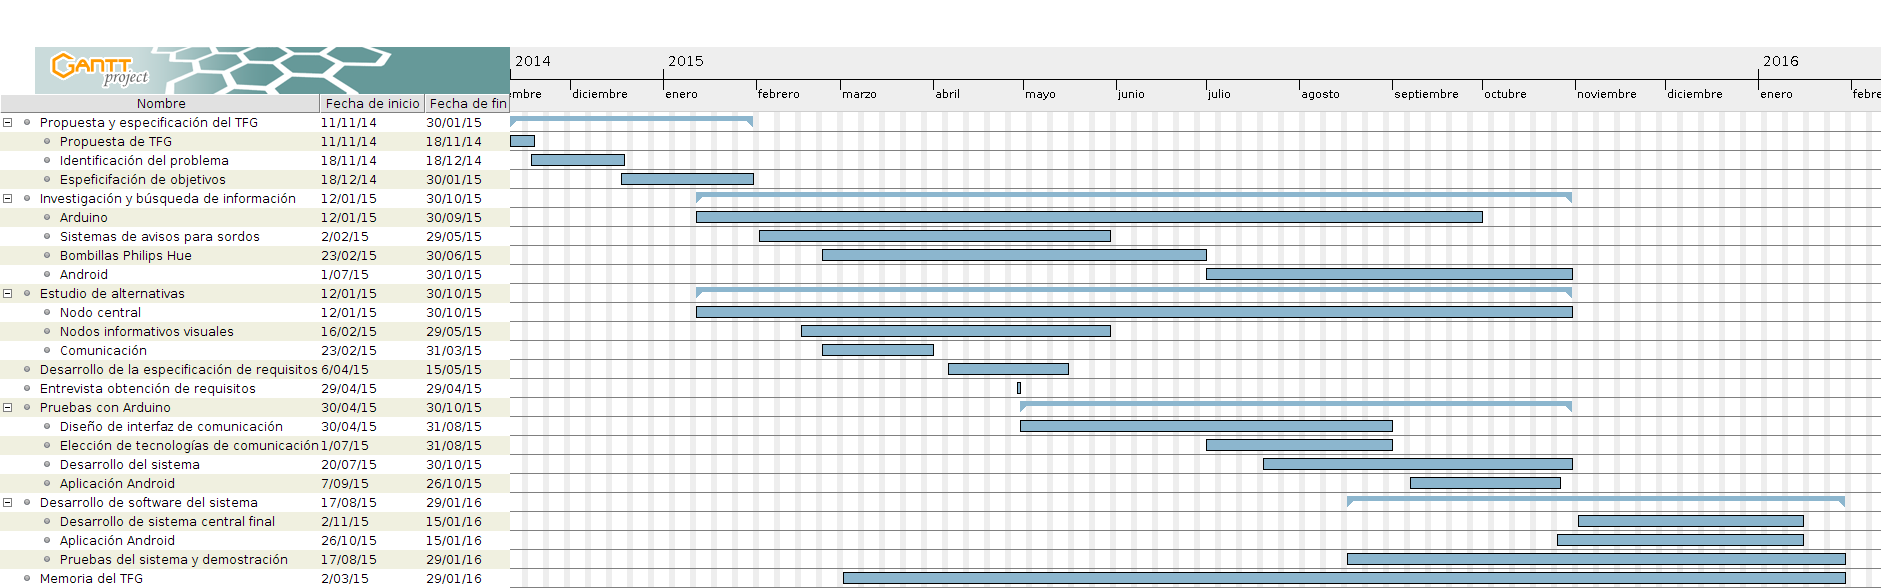
\includegraphics[width=1.15\textwidth,angle=90]{diagramagantt.png}}
        \caption{Diagrama de Gantt de la planificación temporal del Proyecto}
        \label{diagramagantt}
\end{figure}

\clearpage